\subsection{07-80-80-1000-QUICK-SECOND-008-008}
\label{subsec:solution_07}

Considering just only the results obtained for $Re = 1000$, it is easy to see how \texttt{07-80-80-1000-QUICK-SECOND-008-008} is the one that better approximates the exact solution reported by Ghia et al. \cite{Ghia1982HighReSF}.

In the following figure we report all the data results obtained for the simulation runned with the following parameters:

\begin{table}[H]
    \centering
    \begin{tabular}{|c|c|}
        \hline
        \textbf{Variable} & \textbf{Value} \\ \hline
        Re                & 1000           \\
        Nx                & 80             \\
        Ny                & 80             \\
        $\alpha_u$        & 0.08           \\
        $\alpha_v$        & 0.08           \\
        Convection scheme & QUICK          \\
        Diffusion scheme  & SECOND         \\\hline
    \end{tabular}
    \caption{Parameters for simulation 07.}
    \label{tab:parameters_for_comparison}
\end{table}

\begin{figure}[H]
    \centering
    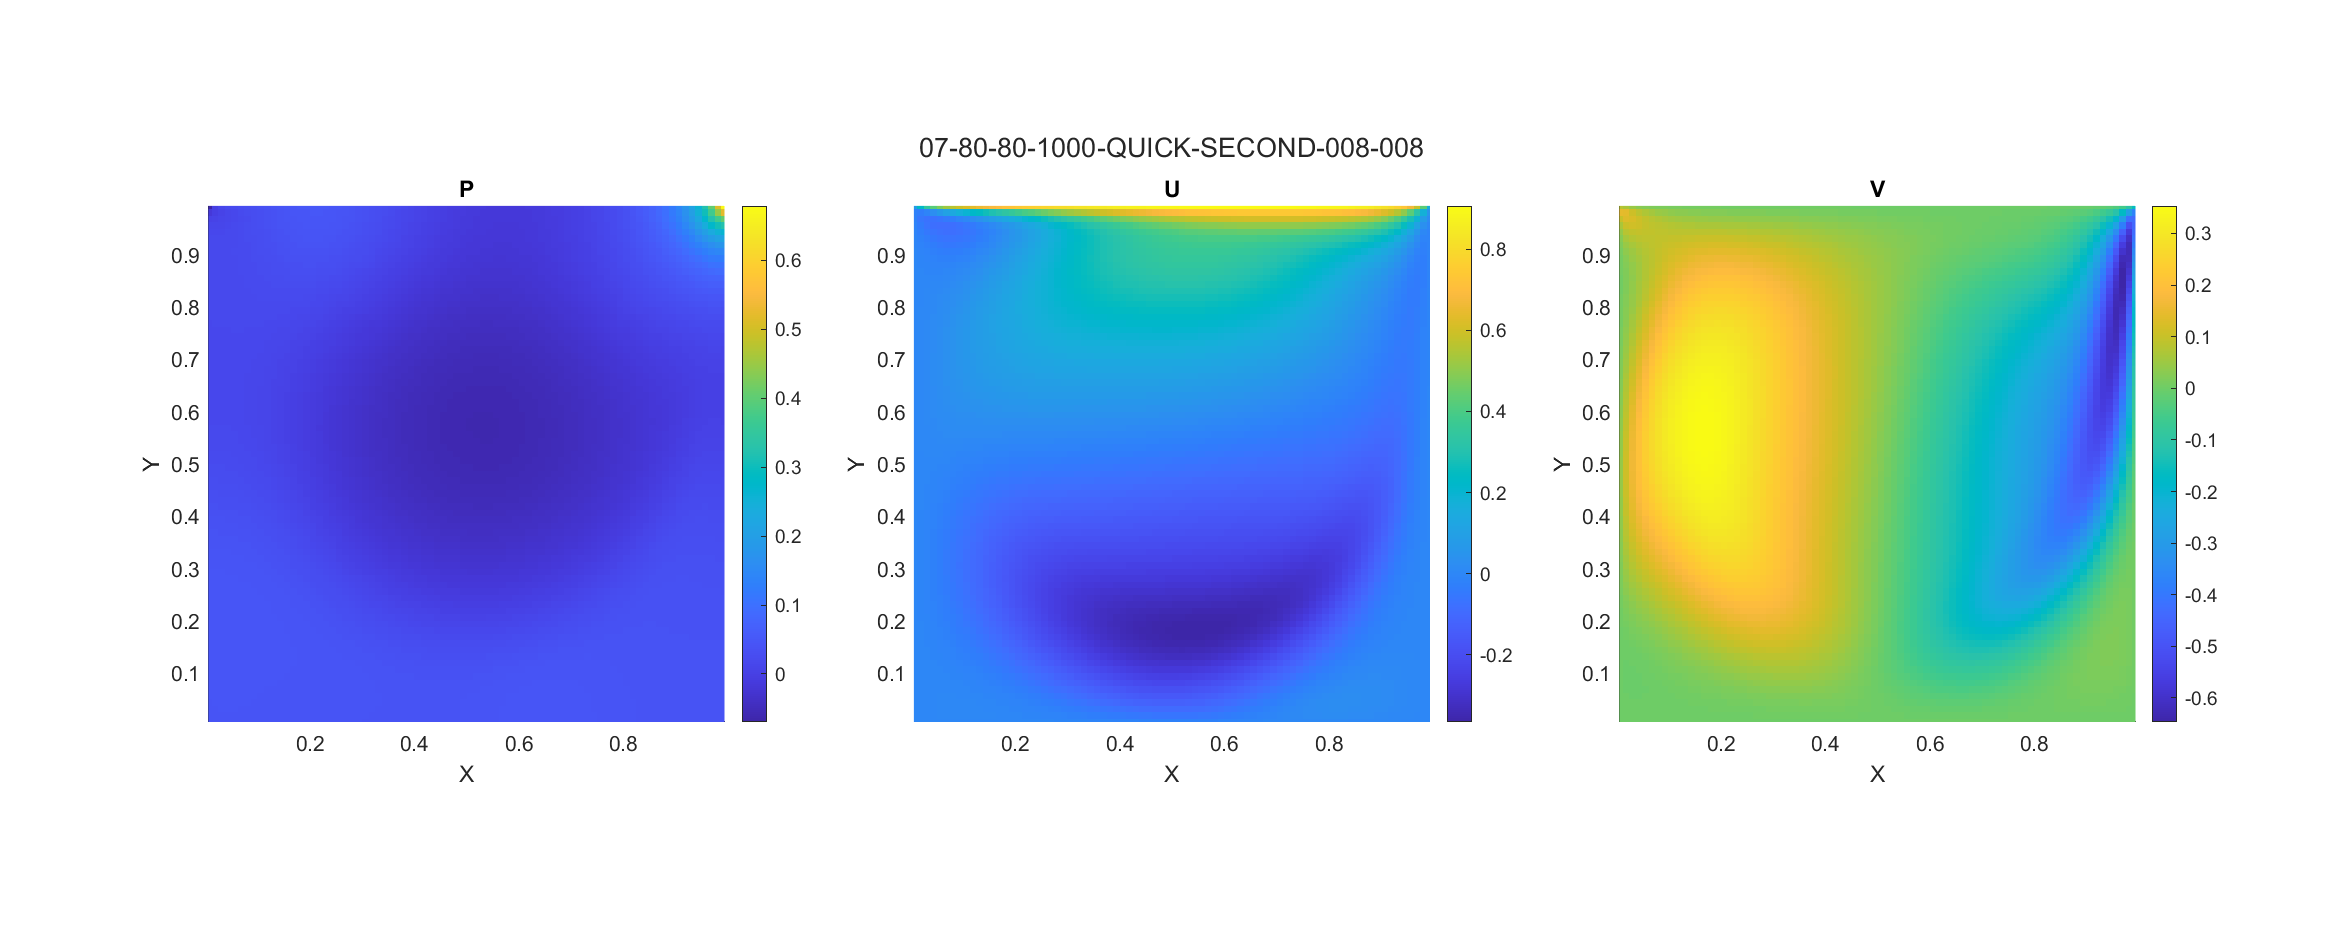
\includegraphics[width=\textwidth]{./img/states/07-80-80-1000-QUICK-SECOND-008-008}
    \caption{Final state of the simulation 07.}
    \label{fig:final_state_07}
\end{figure}

\begin{figure}[H]
    \centering
    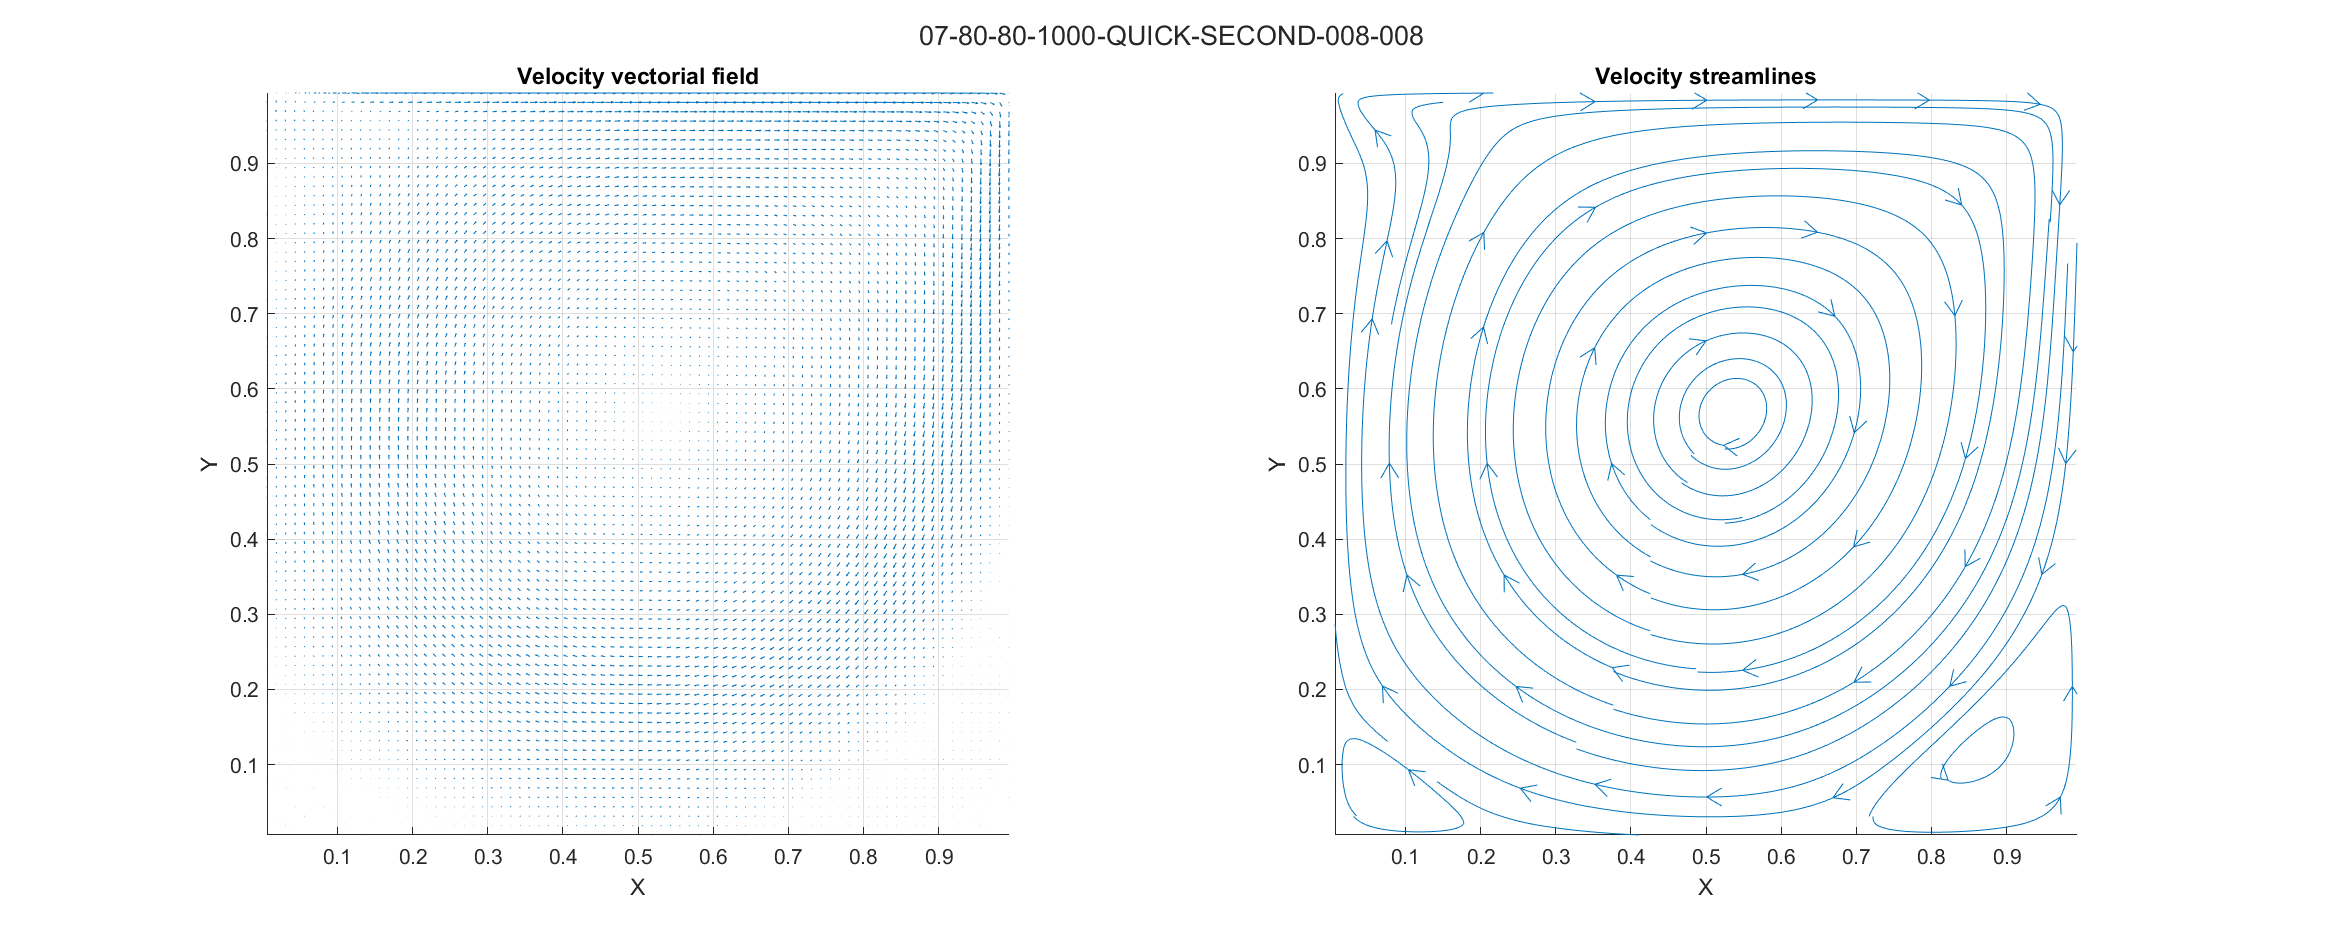
\includegraphics[width=\textwidth]{./img/streamline/07-80-80-1000-QUICK-SECOND-008-008}
    \caption{Streamlines of the simulation 07.}
    \label{fig:streamlines_07}
\end{figure}
